\documentclass{llncs}
\usepackage{times}
\usepackage[T1]{fontenc}

% Comentar para not MAC Users
% \usepackage[applemac]{inputenc}

\usepackage{a4}
%\usepackage[margin=3cm,nohead]{geometry}
\usepackage{epstopdf}
\usepackage{graphicx}
\usepackage{fancyvrb}
\usepackage{amsmath}
\usepackage[backend=biber]{biblatex}
\addbibresource{references.bib}
%\renewcommand{\baselinestretch}{1.5}

\begin{document}
\mainmatter
\title{Uma pesquisa sobre Software Defined Networking}

\titlerunning{Pesquisa sobre SDN}

\author{Miguel Cruz \and Dinis Peixoto \and João Tomás}

\authorrunning{Miguel \and Dinis \and Tomas}

\institute{
University of Minho, Department of  Informatics, 4710-057 Braga, Portugal\\
e-mail: \{a108574, a108566, a108656\}@alunos.uminho.pt
}

\date{}

\maketitle
\begin{abstract}
    \textit {Software Defined Networking} (SDN) é uma nova abordagem de redes que visa simplificar a sua gestão e permitir a inovação através de redes dinâmicas e programáveis,  revolucionando a arquitetura estática das redes tradicionais, descentralizadas e complexas. 
    O objetivo do SDN é melhorar o controlo da rede, permitindo que as empresas e os fornecedores de serviços respondam rapidamente às mudanças nos requisitos do negócio, possibilitando que um administrador molde o tráfego a partir de uma consola de controlo centralizada sem tocar em switches individuais. Conseguindo alterar as regras de qualquer switch de rede quando necessário – priorizando, despriorizando ou até mesmo bloqueando pacotes específicos com um nível de controlo muito granular.
    Isto é especialmente útil numa arquitetura *multi-inquilino* de \textit {cloud computing}  porque permite ao administrador gerir as cargas de tráfego de forma flexível e mais eficiente.
\end{abstract}

\section{Introdução}

\paragraph{} O crescimento exponencial das *\textit {information and communication technologies} (ICT), particularmente, \textit {cloud computing}, a automação de redes e as redes de \textit {data centers}, é catalisada pela integração de sistemas baseados no SDN. \cite{paper1}
 Com a globalização do digital e o aumento do volume de dispositivos conectados, as arquiteturas de redes tradicionais descentralizadas, que dependem de \textit {hardware} especializado, revelaram-se ineficientes face à necessidade de flexibilidade e de escalabilidade. 
 Neste medida, as redes tradicionais oferecem pouco flexibilidade na gestão do tráfego, bem como incapacidade na resposta às novas exigências computacionais, tais como a baixa latência ou a segmentação de rede. 
 Em contraste, o SDN é uma abordagem inovadora que visa simplificar o tráfego através de redes dinâmicas e programáveis. 
 Com a centralização via \textit {software}, os administradores podem moldar as condições da rede conforme a necessidade, otimizando a utilização de recursos, bem como melhorando a qualidade de serviço (QoS).
 \paragraph{}
Complementarmente, o SDN define-se pelas seguintes características. Primeiramente, a capacidade de desassociar o plano de dados do plano de controlo. \cite{paper3}
 Em segundo lugar, o SDN possui um plano de controlo indefinido, o que permite que seja controlado por um único \textit {software}.
 Por conseguinte, o plano de controlo do SDN estende o seu controlo sobre os elementos do plano de dados da rede, por meio do OpenFlow, programa de interface mais utilizado mundialmente.
 Paralelamente, a arquitetura do SDN providencia que um administrador visione a rede globalmente, mas também que faça alterações globalmente.
 \paragraph{}
Neste trabalho, procuramos apresentar a definição de SDN, bem como a sua arquitetura, aliada aos desenvolvimentos existente à data do SDN, bem como abordagens que visionem o desenvolvimento do SDN.
 O trabalho está organizado da seguinte forma. Na segunda secção, apresentaremos uma definição de SDN, a par dos seus benefícios.
 Nas três secções seguintes, apontaremos prospecções de futuros desenvolvimentos possíveis do SDN. 
 Particularmente, na secção três indicaremos otimizações dos controladores SDN, já a secção quatro demonstra um sistema híbrido do SDN e as \textit {legacy networks}, e a secção cinco exibe o desempenho do SDN em larga escala, bem como a sua prospecção face às otimizações mencionadas anteriormente. 
 E, uma sucinta conclusão, que engloba o as implementações atuais do SDN, mas também uma antevisão das implementações futuras, e dos seus benefícios, na secção seis.
 \paragraph{}
\section{SDN: definição e benefícios}
\paragraph{}
Devido à sua emergência, o SDN ainda não dispõe uma definição consensual.
Nesta secção, iremos primeiramente apresentar a mais definição mais creditada, e posteriormente, os benefícios do SDN.
\subsection{Definição de SDN}
\paragraph{}
De acordo com a Open Networking Foundation (ONF), \textit{Software Defined Networking} (SDN) é uma arquitetura de redes dinámica, controlável, econômica e flexível, tornando-a ideal para os usos de banda larga das aplicações atuais. 
Esta arquitetura desassocia as funções de controlo e encaminhamento da rede, possiblitando que o controlo da rede seja diretamente programável. \cite{fundation2012software}
\paragraph{}
Convergentemente, o ONF dispõe de um modelo de referẽncia do SDN, como ilustrado na figura \ref{fig:controller}
\begin{figure}
\begin{center}
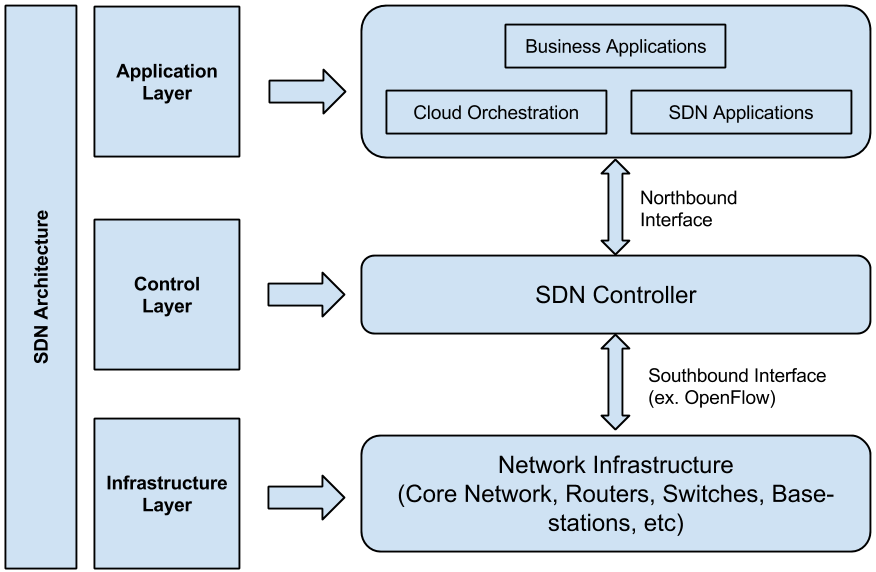
\includegraphics[scale=0.40]{figura1.png} 
\end{center}
\caption{\label{fig:controller}Modelo de Referência do SDN, segundo a ONF.}
\end{figure} 
\paragraph{}

\subsection{Benefícios do SDN}

\section{Optimização de controladores SDN}

\section{Integração de SDN com redes de legado}

\section{Desempenho em implementações em larga escala}

%UNCOMMENT se necess�rio
%De acordo com o ilustrado na Figura~\ref{fig:controller}
%% Exemplo para inser��o de uma figura
%\begin{figure}
%\begin{center}
%\includegraphics[scale=0.40]{figura.pdf} 
%\end{center}
%\caption{\label{fig:controller}Architecture of the unified QoS metric fuzzy controller.}
%\end{figure} 

%According to Table~\ref{tab:TabelaExemplo}...

% Exemplo de uma tabela com duas colunas
%\begin{figure}
%\centering
%\begin{tabular}{|c|c|}\hline
%(a) Delay and jiiter & (b) Delay and loss \\ \hline

%(c) Delay and throughput & (d) Jitter and loss \\ \hline

%(e) Jitter and throughput & (f) Loss and throughput \\ \hline
%\end{tabular}
%\caption{\label{tab:TabelaExemplo}Tabela exemplo.}
%\end{figure}

%\section{Simulation Scenario}

\section{Conclusões}
Neste trabalho...

\printbibliography

\end{document}